% !TEX options=--shell-escape
% Thesis template by Julian Lueken

% Optimized for literature management with JabRef + BibLaTeX

% Change user settings:
%	"keep_focus": true, --> false, to remove the annoying pop ups
%	"use_biblatex": false,
%	"builder": "traditional" --> "basic", to use biber on every compilation
\documentclass[a4paper, 11pt]{report}

% Packages
%% Input encoding
\usepackage[T1]{fontenc}
\usepackage{lmodern}
%%\usepackage[utf8]{inputenc}

%% Syntax
\usepackage{ifthen}

%% Languages and symbols
\usepackage[main=english]{babel}
\usepackage{extarrows}
\usepackage{marvosym}

%% AMS packages
\usepackage{amssymb}
\usepackage{amsmath}
\usepackage{amsthm}

%% Citations and references
\usepackage[style=alphabetic, backend=biber]{biblatex} 
\usepackage[hidelinks]{hyperref}
\usepackage{csquotes}
\usepackage{nameref}
\usepackage{cleveref}
\usepackage{listings}

%% Page geometry
\usepackage[onehalfspacing]{setspace}
\usepackage[top=30mm, left=25mm, right=25mm, bottom=20mm]{geometry}
\usepackage{titlesec}

%% Figures and graphics
\usepackage{graphicx}
\usepackage{xcolor}
\usepackage{colortbl}
\usepackage{subcaption}
\usepackage{tikz}
\usepackage{float}
\usepackage{svg}

%% Pseudo-code
\usepackage{algorithm}
\usepackage[noend]{algpseudocode}

%% Testing
\usepackage{lipsum}

%% Package settings
%%% BibLaTeX resource (JabRef output file)
\addbibresource{../bibtex/bibliography.bib}

%%% Hyperref options
\hypersetup{hypertexnames=false}

%%% Listings options (for writing code in LaTeX)
\lstset{numbers=left, numberstyle=\tiny, numbersep=5pt}
\lstset{language=Python}

%%% AMS environment definitions
\theoremstyle{definition}
\newtheorem{definition}{Definition}[section]
\newtheorem{example}[definition]{Example}
\newtheorem{theorem}[definition]{Theorem}
\newtheorem{corollary}[definition]{Corollary}
\newtheorem*{remark}{Remark}
\newenvironment{myAbstract}{\section*{Abstract}}{}

%%% Special formatting
\renewcommand{\emph}[1]{\textit{#1}}
\newcommand{\mytitle}[1]{\LARGE{#1}\normalsize\\[0.3em]}
\newcommand{\titlespace}{\vspace{2em}}
\newcommand{\smallspace}{\vspace{1em}}
\newcommand{\hugespace}{\vspace{17em}}
\newcommand{\logoheight}{4em}

%% Special formatting for pesudocode
\algblock{Input}{EndInput}
\algnotext{EndInput}
\algblock{Output}{EndOutput}
\algnotext{EndOutput}
\newcommand{\Desc}[2]{\State \makebox[12em][l]{#1}#2}


\begin{document}

% Chapter format
\titleformat{\chapter}[hang]{\normalfont\huge\bfseries}{\thechapter}{0.75em}{\huge\bfseries}
\titlespacing*{\chapter}{0em}{0em}{1em}

% Title page
\pagenumbering{gobble}
\newgeometry{top=35mm, left=20mm, right=20mm, bottom=10mm}
\begin{titlepage}
	\begin{center}
		\begin{minipage}{.49\textwidth}
			\flushleft
			
\includegraphics[height=\logoheight]{../assets/formal/logo_gau.png}
		\end{minipage}
		\begin{minipage}{.49\textwidth}
			\flushright
			
\includegraphics[height=\logoheight]{../assets/formal/logo_dlr.png}	
		\end{minipage}
		\begin{minipage}{.49\textwidth}

			\begin{center}
				\vspace{2cm}
				Master's thesis in\\
				Applied Computer Science\\
				\titlespace
				\mytitle{CoolingGen}
				A parametric 3D-modeling software for turbine blade cooling geometries using NURBS\\
				\titlespace
				\today\\
				\hugespace
				Institute for Numerical and Applied Mathematics at the Georg-August-University Göttingen\\
				\titlespace
				Institute for Propulsion Technology at the German Aerospace Center in Göttingen\\
				\titlespace
				Bachelor's and master's theses at the Center for Computational Sciences at the Georg-August-University Göttingen\\
				\titlespace
				Julian Lüken\\
				\texttt{julian.lueken@dlr.de}\\
			\end{center}
		\end{minipage}
	\end{center}
\end{titlepage}
\pagebreak

% Address page
\pagestyle{empty}
\restoregeometry
\newgeometry{top=210mm, left=45mm, right=45mm}
\noindent
\begin{tabular}{l}
Georg-August-University Göttingen\\
Institute of Computer Science\\
\end{tabular}\\[1em]
\begin{tabular}{ll}
	\Telefon 	&+49 (551) 39-172000\\
	\FAX 		&+49 (551) 39-14403\\
	\Letter 	&\texttt{office@cs.uni-goettingen.de}\\
\end{tabular}\\[1em]
\begin{tabular}{l}
\texttt{www.informatik.uni-goettingen.de}\\
\end{tabular}\\[1em]
\pagebreak

% Done-it-myself page
\noindent I hereby declare that this thesis has been written by myself and no other resources than those mentioned have been used.\\[0.7em]
\phantom{H}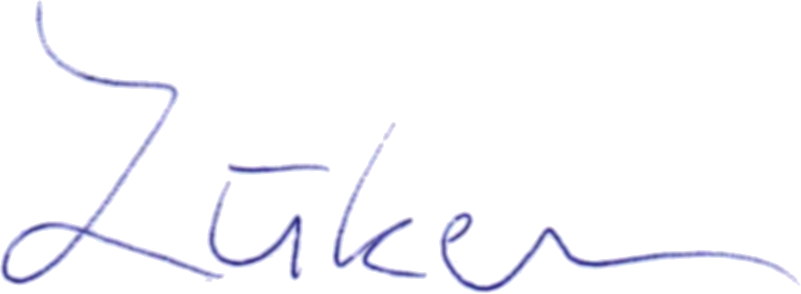
\includegraphics[height=3em]{../assets/formal/sign.png}\\[0.5em]
Göttingen, \today \hspace{2em}
\pagebreak

% Abstract and Zusammenfassung
\restoregeometry
\begin{abstract}
	\thispagestyle{plain}
	\pagenumbering{roman}
	\setcounter{page}{3}
	\lipsum[1-3]
\end{abstract}
\renewcommand{\abstractname}{Zusammenfassung}
\begin{abstract}
	\thispagestyle{plain}
	\pagenumbering{roman}
	\setcounter{page}{4}
	\lipsum[4-6]
\end{abstract}
\pagebreak

% Table of contents
\setcounter{page}{5}
\restoregeometry
\tableofcontents
\pagebreak

% Actual document starts here
\restoregeometry
\pagenumbering{arabic}
\setcounter{page}{1}
\pagestyle{plain}

\chapter{Introduction}
\section{Motivation}
\section{State of the Art}
\section{Problem Statement}

\chapter{Methods}
As stated before, Non-Uniform Rational B-splines (NURBS) are used to model curves and surfaces in CoolingGen. In this chapter we will first introduce Beziér curves. We will then generalize Beziér curves to obtain B-spline objects. Using an embedding map and a projection map, we will find a generalization of B-spline objects, namely NURBS objects. Furthermore, CoolingGen uses special geometric algorithms such as point inversion, curve intersection and curve fillet fitting, which we will also present.

\section{Bézier Curves}
Bézier curves are named after the French engineer Pierre Bézier, who famously utilized them in the 1960s to design car bodies for the automobile manufacturer Renault \cite{Bezier1968}. Today, they are used in a wide variety of vector graphics applications (i.e. in font representation on computers). At first glance, the definition of the Bézier curve might seem cumbersome, but given the mathematical foundation and a few graphical representations, it becomes apparent why they are such a powerful tool in computer-aided design.

\begin{figure}[H]
	\centering
	\begin{subfigure}{0.25\textwidth}
		\includesvg[width=\textwidth]{../python/bezierDifferentDegrees1}
		\caption{Degree $1$.}
	\end{subfigure}
	\begin{subfigure}{0.25\textwidth}
		\includesvg[width=\textwidth]{../python/bezierDifferentDegrees2}
		\caption{Degree $2$.}
	\end{subfigure}
	\begin{subfigure}{0.25\textwidth}
		\includesvg[width=\textwidth]{../python/bezierDifferentDegrees3}
		\caption{Degree $3$.}
	\end{subfigure}
	\caption{Beziér curves of different degrees (orange) and their control points (blue).}
\end{figure}

\subsection{Definition}
\begin{definition}
	The \emph{Bernstein basis polynomials} of degree $n$ on the interval $[t_0,t_1]$ are defined as
	\begin{equation}\label{eq:bernsteinbasisdef}
		b_{n,k,[t_0, t_1]}(t) := \frac{\binom{n}{k} (t_1-t)^{n-k}(t-t_0)^k}{(t_1-t_0)^n},
	\end{equation}
	for $k \in \{0,\dots, n\}$.
\end{definition}

\begin{definition}
	Let $V$ a vector space. A \emph{Bézier curve} of degree $n$ is a parametric curve $B_{P,[t_0, t_1]}: [t_0, t_1] \rightarrow V$ that has a representation
	\begin{equation}\label{eq:bezierdef}
		B_{P, [t_0, t_1]}(t) = \sum_{k=0}^n b_{n,k,[t_0, t_1]}(t) P_k = \sum_{k=0}^n \frac{\binom{n}{k} (t_1-t)^{n-k}(t-t_0)^k}{(t_1-t_0)^n} P_k.
	\end{equation}
	We call the elements of the set $P = \{P_0, P_1, \dots, P_n\} \subset V$ the \emph{control points} of $B_P$.
\end{definition}

\begin{remark}
	Let $t_0 = 0$ and $t_1 = 1$. Then \ref{eq:bezierdef} simplifies to
	\begin{equation}
		b_{n,k}(t) := b_{n,k,[0,1]}(t) = \binom{n}{k} (1-t)^{n-k}t^k
	\end{equation}
	and \ref{eq:bernsteinbasisdef} simplifies to
	\begin{equation}\label{eq:bezierdefshort}
		B_P(t) := B_{P,[0,1]}(t)= \sum_{k=0}^n \binom{n}{k} (1-t)^{n-k}t^k P_k.
	\end{equation}
	This case is the only case considered in this thesis. We also set the vector space $V$ to be $\mathbb{R}^3$ unless specified otherwise.
\end{remark}

\subsection{De Casteljau's Algorithm}

The computation of Equation \ref{eq:bezierdefshort} is usually performed using de Casteljau's algorithm. This is because the algorithm yields a simple implementation and lower complexity than straightforwardly computing Equation \ref{eq:bezierdefshort}. The algorithm was proposed by Paul de Faget de Casteljau for the automobile manufacturer Citroën in the 1960s.

\begin{algorithm}[H]
	\begin{algorithmic}[1]
		\Input
			\Desc{$P = \{P_0, P_1, ..., P_n\}$}{set of control points}
			\Desc{$t$}{real number}
		\EndInput
		\Output
			\Desc{$P^{(n)}_0 = B_P(t)$}{the point on the Beziér curve w.r.t. to $t$}
		\EndOutput

		\caption{de Casteljau's algorithm}\label{alg:decasteljaualgo}
		\Procedure{deCasteljau}{$P, t$}
			\State $P^{(0)} \gets P$
			\For {$j = 1, 2, ..., n$}
				\For {$k = 0, 1, ..., n-j$}
					\State $P^{(j)}_k \gets (1-t) \cdot P^{(j-1)}_k + t \cdot P^{(j-1)}_{k+1}$
				\EndFor
			\EndFor
			\Return $P^{(n)}_0$
		\EndProcedure
	\end{algorithmic}
\end{algorithm}

\begin{theorem}
	Algorithm \ref{alg:decasteljaualgo} computes $B_P(t)$.
\end{theorem}
\begin{proof}
	By induction. Let $n = 1$. Then
		$$ P_0^{(1)} = (1-t) \cdot P_0 + t \cdot P_1.$$
	By employing the induction hypothesis
		$$ P_j^{(n)} = \sum_{k=j}^{n+j} \binom{n}{k} (1-t)^{n-k}t^k P_{j+k}$$
	for some $n \in \mathbb{N}$, we can infer that
	\begin{align*}
		P_0^{(n+1)}	&= (1-t) \cdot P_0^{(n)} + t \cdot P_1^{(n)} \\
					&= (1-t) \cdot \sum_{k=0}^{n} \binom{n}{k} (1-t)^{n-k}t^k P_{k} + t \cdot \sum_{k=1}^{n+1} \binom{n}{k} (1-t)^{n-k}t^k P_{k+1} \\
					&= \sum_{k=0}^{n+1} \binom{n+1}{k} (1-t)^{n+1-k}t^k P_{k},
	\end{align*}
	which is equal to $B_P(t)$ for degree $n+1$.
\end{proof}

A visual representation of Algorithm \ref{alg:decasteljaualgo} yields a triangular scheme. To compute one point on a Beziér curve $B_P$ with degree $n$, one has to perform $\frac{n^2-n}{2}$ vector additions and $n^2-n$ scalar multiplications.

\begin{figure}[H]
	\centering
	\begin{subfigure}{0.49\textwidth}
		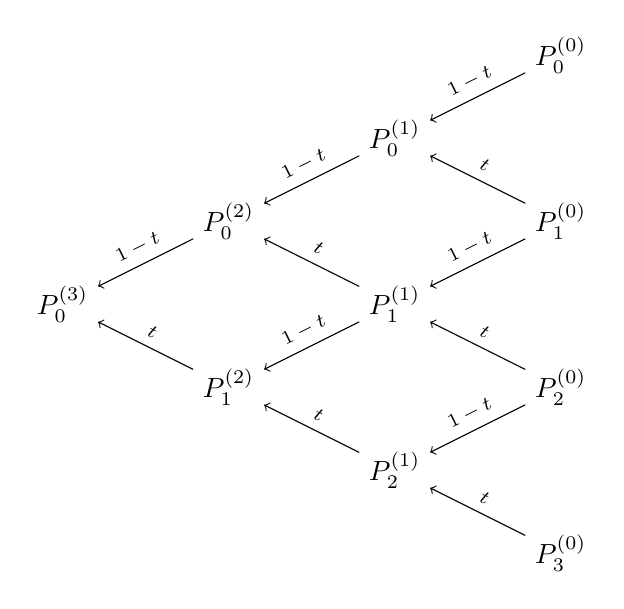
\begin{tikzpicture}
			\def\dx{60pt}
			\def\dy{30pt}

			\pgfmathsetmacro{\degree}{3}

			% Make nodes
			\newcounter{i}
			\newcounter{j}

			\node (\arabic{i}) at (0,0) {$P^{(\degree)}_0$};
			\stepcounter{i}

			\foreach \x in {1, ..., \degree} {
				\pgfmathsetmacro{\xstep}{\x-2}

				\setcounter{j}{0}
				\foreach \y in {\x, \xstep, ..., -\x} {
					\node (\arabic{i}) at (\x*\dx, \y*\dy) {$P^{(\pgfmathint{\degree-\x}\pgfmathresult)}_{\arabic{j}}$};
					\stepcounter{i}
					\stepcounter{j}
				}
			}
			
			% Make arrows
			\newcounter{z}
			\newcounter{a}
			\newcounter{b}
			\pgfmathsetmacro{\maxx}{\degree}
			\foreach \x in {1,...,\degree}{
				\foreach \y in {1,...,\x}{
					
					\setcounter{a}{\arabic{z}}
					\addtocounter{a}{\x}

					\setcounter{b}{\arabic{z}}
					\addtocounter{b}{\x}
					\stepcounter{b}
					
					\draw [<-] (\arabic{z}) -- (\arabic{a}) node[above, midway, sloped] {\scriptsize $1-t$};
					\draw [<-] (\arabic{z}) -- (\arabic{b}) node[above, midway, sloped] {\scriptsize $t$};
					
					\stepcounter{z}
				}
			}
		\end{tikzpicture}
		\caption{Algorithmic visualization.}
	\end{subfigure}
	\hfill
	\begin{subfigure}{0.49\textwidth}
		\includesvg[width=\textwidth]{../python/deCasteljauVisual}
		\caption{Geometric visualization of $B_P(\frac{3}{5})$.}
	\end{subfigure}
	\caption{Visual representations of de Casteljau's algorithm.}
	\label{fig:decasteljautriangle}
\end{figure}

Interestingly, the representation of the algorithm in Figure \ref{fig:decasteljautriangle} also gives rise to an intuitive visualization of the geometric shape of the Beziér curve $B_P$. For all $i \in \{0, ..., n\}$ and all $j \in \{0, ..., n-i\}$, the point $P^{(i+1)}_j$ is the convex combination (always w.r.t. $t$) of $P^{(i)}_j$ and $P^{(i)}_{j+1}$. Thus $P^{(i+1)}_j$ always lies on the line segment between $P^{(i)}_j$ and $P^{(i)}_{j+1}$, as can be observed in the example in Figure \ref{fig:decasteljautriangle}.

\subsection{Properties}
Other than being remarkably intuitive, Beziér curves have a lot of properties which make them convenient. In computer-aided design software, most graphical user interfaces rely on the principle of letting the user interactively drag and drop the control points with a mouse, granting them control over the shape of Beziér curve. The following theorems further illustrate why this is a good idea.

\begin{theorem}
	$B_P(0) = P_0$ and $B_P(1) = P_n$.
\end{theorem}
\begin{proof}
	Explicit computation yields
		$$B_P(0) = \sum_{k=0}^n \binom{n}{k} t^k P_k = \binom{n}{0} P_0 = P_0$$
	and
		$$B_P(1) = \sum_{k=0}^n \binom{n}{k} (1-t)^{n-k} P_k = \binom{n}{n} P_n = P_n.$$
\end{proof}

\begin{theorem}
	Let $T \in \mathbb{R}^{3 \times 3}$. Then $B_{TP}(t) = TB_P(t)$ where $TP := \{TP_0, TP_1, ..., TP_n\}$.
\end{theorem}
\begin{proof}
	For all $t \in [0, 1]$ we can directly compute
		$$TB_P(t) = \sum_{k=0}^n \binom{n}{k} (1-t)^{n-k}t^k TP_k = B_{TP}(t).$$
\end{proof}

\begin{theorem}
	$B_P(t)$ lies in the convex hull of $P$ for all $t \in [0,1]$.
\end{theorem}
\begin{proof}
	By the algorithm of de Casteljau (\ref{alg:decasteljaualgo}), we know that $P^{(i)}_j = (1-t) \cdot P^{(i-1)}_j + t \cdot P^{(i-1)}_{j+1}$ for all $t \in [0, 1]$. Therefore, $P^{(i)}$ lie in the convex hull of $P^{(i-1)}$. But then $B_P(t) = P^{(n)}_0$ always lies in the convex hull of $P^{(0)} = P$ by induction.
\end{proof}

Simple as their appearance may be, Beziér curves fall short of representing some of the most common geometric shapes. Given a finite number of control points, we can never make $B_P(t)$ a circular arc, although a circle has a very simple parametric form. One of their greatest perks, the ability to describe a shape with just a handful of control points, is their greatest shortcoming at the same time. This is most likely the reason why Beziér curves are not the state of the art in technical engineering applications. However, Beziér curves certainly do provide an intuition for Non-Uniform Rational B-Splines or NURBS, which is their prevailing counterpart.

\section{Non-Uniform Rational B-splines (NURBS)}
NURBS are a state of the art tool for curve and surface modelling. There is a somewhat common joke that describes the acronym NURBS as \emph{"Nobody Understands Rational B-Splines"} (source?). In this section, we invalidate this punch line. First of all, we discuss B-splines, then we construct B-spline curves and then we apply simple transformations to the B-spline curve to acquire NURBS.

\subsection{Definition}
Similarly to how Beziér curves are defined on the Bernstein polynomial basis, NURBS are defined on basis functions called basis splines (or more commonly B-splines), which are recursively defined on a \emph{knot sequence} $(t_m)_{m=-\infty}^{\infty} \subset \mathbb{R}$ with $t_{m} \leq t_{m+1}$ for all $m \in \mathbb{Z}$.

\begin{definition}
	The \emph{B-splines of degree $0$} on a knot sequence $(t_m)$ are defined as
	\begin{equation}
		N^{(t_m)}_{1,k}(t) :=
		\begin{cases}
			1 & \text{if } t \in [t_k, t_{k+1}),\\
			0 & \text{else.}
		\end{cases}
	\end{equation}
	The \emph{B-splines of degree $p-1$} with $p > 1$ are given by the \emph{Cox-de-Boor recursion formula}
	\begin{equation}\label{eq:coxdeboorrec}
		N_{p,k}^{(t_m)}(t) := \omega^{(t_m)}_{p-1, k}(t) \, N^{(t_m)}_{p-1, k}(t) + (1-\omega^{(t_m)}_{p-1, k+1}(t)) \, N^{(t_m)}_{p-1, k+1}(t),
	\end{equation}
	where
	\begin{equation}
		\omega^{(t_m)}_{p,k}(t) := 
		\begin{cases}
			\frac{t-t_k}{t_{k+p} - t_k} &\text{if } t_{k+p} \neq t,\\
			0 							&\text{else.}
		\end{cases}
	\end{equation}
\end{definition}

\begin{remark}
	Instead of $N_{p,k}^{(t_m)}$ we write $N_{p,k}$ and explicitly refer to $(t_m)$ when necessary. We restrict the domain of definition of $N_{p,k}$ to $[0, 1)$ by setting $\lim_{m \to -\infty} t_m = 0$ and $\lim_{m \to \infty} t_m = 1$.
\end{remark}

\begin{definition}
	Let $V$ a vector space. A \emph{B-spline curve} of degree $p-1$ over a set of control points $P = \{P_0, P_1, ... P_n\} \subset V$ and a knot sequence $(t_m)$ is defined as $$ S_P(t) = \sum_{k=0}^{n} N_{p,k}(t) P_k.$$
\end{definition}

\begin{definition}\label{def:nurbs}
	A \emph{NURBS curve} $C_P(t)$ of degree $p-1$ with the control points $P = \{P_0, P_1, ..., P_n\} \subset V$, the control weights $w = (w_0, w_1, ... w_n) \subset \mathbb{R}$ and a knot sequence $(t_m)$ is defined as
	\begin{equation}
		C_P(t) = \frac{\sum_{k=0}^n N_{p,k}(t) w_k P_k}{\sum_{k=0}^n N_{p,k}(t) w_k}.
	\end{equation}
\end{definition}

\begin{remark}
	Let $\dim V = d$. A NURBS curve can alternatively be understood as a projection of a B-spline curve on a transformed set of control points. For this purpose we define the embedding into the weighted vector space
		$$\Phi_w: V \rightarrow V \times \mathbb{R}$$
	that maps each control point $P_k = (p_1, ..., p_d) \in V$ onto $(w_k p_1, ..., w_k p_d, w_k) \in V \times \mathbb{R}$.
	We also have to define the projection map
		$$\Phi^\dagger: V \times \mathbb{R} \rightarrow V$$ 
	that maps each point on the B-spline curve $S_{\Phi(P)}(t) = (s_1, ..., s_d, s_{d+1})$ onto $(\frac{s_1}{s_{d+1}}, ..., \frac{s_d}{s_{d+1}})$.
	We can then define the NURBS curve as
			$$ C_P(t) = \Phi^\dagger(S_{\Phi_w(P)}(t))$$ 
	which we will make use of later on.
\end{remark}

\begin{theorem}
	Let $w \equiv 1$. Then $S_P \equiv \Phi^\dagger(S_{\Phi_w(P)})$. In other words, NURBS curves are a generalization of B-spline curves.
\end{theorem}
\begin{proof}
	Since in this case $\Phi_w((p_1, ..., p_d)) = (p_1, ..., p_d, 1)$, we have that $\Phi^\dagger(S_{\Phi_w(P)}(t)) = \Phi^\dagger(\Phi_w(S_P(t))) = S_P(t)$.
\end{proof}

Now that we have defined B-spline curves and NURBS curves, we can define B-spline surfaces and NURBS surfaces in a similar manner. To do this, we require a grid of knots represented by two knot sequences $(u_m)_{m=-\infty}^{\infty}$ and $(v_m)_{m=-\infty}^{\infty}$ which satisfy the same conditions as $(t_m)$ did before. Instead of a one-dimensional set of control points, the surface definition relies on a two-dimensional set of control points. Notice that this grants us control 

\begin{definition}
	A \emph{B-spline surface} $S_P(u,v)$ of degree $(p-1, q-1)$ over a set of control points $P = \{P_{i,j} : (i,j) \in \{0,1,...,n_u\} \times \{0,1,...,n_v\}\} \subset V$ on the knot grid $(u_m), (v_m)$ is defined as
		$$ S_P(u,v) = \sum_{k_u=0}^{n_u} \sum_{k_v=0}^{n_v} N_{p,k_u}(u) N_{q,k_v}(v) P_{k_u,k_v},$$
	where $N_{p,k_u}(u) := N_{p,k_u}^{(u_m)}(u)$ and $N_{q,k_v}(v) := N_{q,k_v}^{(v_m)}(v)$.
\end{definition}

\begin{definition}
	A \emph{NURBS surface} $C_P(u,v)$ of degree $(p-1, q-1)$ over a set of control points $P = \{P_{i,j} : (i,j) \in \{0,1,...,n_u\} \times \{0,1,...,n_v\}\} \subset V$, the control weights $w = \{w_{i,j} : (i,j) \in \{0,1,...,n_u\} \times \{0,1,...,n_v\}\} \subset \mathbb{R}$ and the knot grid $(u_m), (v_m)$ is defined as
		$$ C_P(u,v) = \frac {\sum_{k_u=0}^{n_u} \sum_{k_v=0}^{n_v} N_{p,k_u}(u) N_{q,k_v}(v) w_{k_u, k_v} P_{k_u,k_v}}{\sum_{k_u=0}^{n_u} \sum_{k_v=0}^{n_v} N_{p,k_u}(u) N_{q,k_v}(v) w_{k_u, k_v}},$$
	where $N_{p,k_u}(u) := N_{p,k_u}^{(u_m)}(u)$ and $N_{q,k_v}(v) := N_{q,k_v}^{(v_m)}(v)$.
\end{definition}

\begin{remark}
	As with NURBS curve, we have the analogous result
		$$ C_P(u,v) = \Phi^\dagger ({S_{\Phi_w(P)}(u,v)}) $$
	for NURBS surfaces.
\end{remark}

The notion of the knot sequence $(t_m)$ is commonly computationally simplified to that of a knot vector $\tau$, since $\tau$ only contains a finite number of elements. For our purposes, we let
	$$\tau = (\underbrace {t_0, ..., t_{p-1}}_{= 0}, t_p, ..., t_n, \underbrace{t_{n+1}, ..., t_{n+p}}_{= 1}),$$
where $t_k = 0$ for $k \in \{0,...,p-1\}$ and $t_k = 1$ for $k \in \{n+1, ..., n+p\}$. We still require the monotony property $t_k \leq t_{k+1}$ for all $k \in \{0, ..., n+p\}$.

\subsection{De Boor's Algorithm}
To efficiently calculate points on a B-spline object, Carl-Wilhelm Reinhold de Boor devised an efficient algorithm, the construction of which demonstrates its correctness. Together with the embedding $\Phi_w$ and the projection $\Phi^\dagger$ from the Remark for Definition \ref{def:nurbs}, this algorithm can also be used to calculate points on a NURBS object.

Let $P = \{P_0, P_1, ..., P_n\}$ a set of control points, $(t_m)$ a knot sequence and $p-1$ the degree of the B-spline curve $S(t)$. Then by the Cox-de-Boor recursion formula, we find
\begin{align*}
	S(t) 	&= \sum_{k=0}^n N_{p,k}(t) \, P_k \\
			&= \sum_{k=1}^n \omega_{p-1,k}(t) \, N_{p-1, k}(t) \, P_k  \; + \; \sum_{k=0}^n \left( 1-\omega_{p-1,k+1}(t) \right) \, N_{p-1, k+1}(t) \, P_k.
\end{align*}
Changing the limits of the second term, we can summarize the two terms as
\begin{align*} 
	S(t) 	&= \sum_{k=1}^n N_{p-1, k}(t) \, \underbrace{\Big[ \omega_{p-1,k}(t) \, P_k  \, + \, \left( 1-\omega_{p-1,k}(t) \right) \, P_{k-1} \Big]}_{=: P_k^{(1)}(t)} \\
			&= \sum_{k=1}^n N_{p-1, k}(t) \, P_k^{(1)}(t).
\end{align*}
Recursively defining
\begin{equation}\label{eq:debooriteration}
	P^{(j)}_k(t) := \begin{cases}
		\omega_{p-j, k} \, P^{(j-1)}_k(t) \, + \, (1-\omega_{p-j, k}) \, P^{(j-1)}_{k-1}(t) 	&\text{if } j > 0,\\
		P_k 																					&\text{else},
	\end{cases}
\end{equation}
we can repeat this process up to $p-2$ more times, finding
$$ S(t) = \sum_{k=p-1}^n N_{1, k}(t) \, P^{(p-1)}_k(t) = P^{(p-1)}_l(t)$$
for $t \in [t_l, t_{l+1})$. We can thus use the recursive definition in Equation \ref{eq:debooriteration} as the key step of our algorithm to compute $S(t)$. It is already clear from this place that the points calculated on a B-spline curve are in fact also a cumultated convex combination of control points, just as it is the case with Beziér curves. As zero-values for $\omega_{i,j}$ (or $1-\omega_{i,j}$) can be completely omitted by checking multiplicity, we arrive at the following algorithm:

\begin{algorithm}[H]
	\begin{algorithmic}[1]
		\Input
			\Desc{$P = \{P_0, P_1, ..., P_n\}$}{set of control points of the B-spline curve}
			\Desc{$\tau = (t_0, t_1, ..., t_{n+p})$}{knot vector of the B-spline curve}
			\Desc{$p-1$}{degree of the B-spline curve}
			\Desc{$t \in [t_0, t_{n+p})$}{real number}
		\EndInput
		\Output
			\Desc{$S_P(t)$}{the point on the B-spline curve w.r.t. to $t$}
		\EndOutput

		\caption{de Boor's algorithm for curves}\label{alg:debooralgo}
		\Procedure{deBoorCurve}{$P, p, \tau, t$}
			\State Find $l$ such that $t \in [t_l, t_{l+1})$
			\State Let $m$ be the multiplicity of $t$ in the knot vector $\tau$
			\State $P^{(0)} \gets P$

			\For {$j = 1, 2, ..., p-m-1$}
				\For {$k = l-p+j+1, ..., l-m$}
					\State $\omega_{p-j,k} \gets \frac{t-t_k}{t_{k+p-j} - t_k}$
					\State $P^{(j)}_k \gets (1-\omega_{p-j,k}) \cdot P^{(j-1)}_{k-1} + \omega_{p-j,k} \cdot P^{(j-1)}_k$
				\EndFor
			\EndFor

			\Return $P^{(p-m-1)}_{l-m} = C_P(t)$
		\EndProcedure
	\end{algorithmic}
\end{algorithm}

\begin{figure}[H]
	\centering
	\begin{subfigure}{0.49\textwidth}
		\begin{tikzpicture}
			\def\dx{65pt}
			\def\dy{30pt}

			\pgfmathsetmacro{\degree}{3}

			% Make nodes
			\setcounter{i}{0}
			\setcounter{j}{0}

			\node (\arabic{i}) at (0,0) {$P^{(\degree)}_l$};
			\stepcounter{i}

			\foreach \x in {1, ..., \degree} {
				\pgfmathsetmacro{\xstep}{\x-2}

				\setcounter{j}{0}
				\foreach \y in {\x, \xstep, ..., -\x} {

					\ifthenelse{\value{j}>0} {
						\node (\arabic{i}) at (\x*\dx, \y*\dy) {$P^{(\pgfmathint{\degree-\x}\pgfmathresult)}_{l-\arabic{j}}$};
					}
					{
						\node (\arabic{i}) at (\x*\dx, \y*\dy) {$P^{(\pgfmathint{\degree-\x}\pgfmathresult)}_l$};
					}
					\stepcounter{i}
					\stepcounter{j}
				}
			}
			
			% Make arrows
			\setcounter{z}{0}
			\setcounter{a}{0}
			\setcounter{b}{0}
			\pgfmathsetmacro{\maxx}{\degree}
			\foreach \x in {1,...,\degree}{
				\foreach \y in {1,...,\x}{
					
					\setcounter{a}{\arabic{z}}
					\addtocounter{a}{\x}

					\setcounter{b}{\arabic{z}}
					\addtocounter{b}{\x}
					\stepcounter{b}
					
					\ifthenelse{\y > 1} {
						\draw [<-] (\arabic{z}) -- (\arabic{b}) node[above, midway, sloped] {\scriptsize $1-\omega_{\pgfmathint{\x}\pgfmathresult, l-\pgfmathint{\y-1}\pgfmathresult}$};
						\draw [<-] (\arabic{z}) -- (\arabic{a}) node[above, midway, sloped] {\scriptsize $\omega_{\pgfmathint{\x}\pgfmathresult, l-\pgfmathint{\y-1}\pgfmathresult}$};
					}
					{
						\draw [<-] (\arabic{z}) -- (\arabic{b}) node[above, midway, sloped] {\scriptsize $1-\omega_{\pgfmathint{\x}\pgfmathresult, l}$};
						\draw [<-] (\arabic{z}) -- (\arabic{a}) node[above, midway, sloped] {\scriptsize $\omega_{\pgfmathint{\x}\pgfmathresult, l}$};
					}

					\stepcounter{z}
				}
			}
		\end{tikzpicture}
		\caption{Visualization of de Boor's algorithm on a curve $S_P(t)$ with degree $3$, where $t$ does not appear in the knot vector $\tau$ (in other words, $m=0$.}
	\end{subfigure}
	\hfill
	\begin{subfigure}{0.49\textwidth}
		\centering
		\includesvg[width=0.99\textwidth]{../python/nurbsCurveExample}
		\caption{Degree $3$ NURBS curve $\Phi^\dagger(S_{\Phi_w(P)}(t))$  for different values of a single entry of the control weight vector $w$.}
	\end{subfigure}
	\caption{Calculating points on a NURBS curve.}
	\label{fig:debooralgo}
\end{figure}

To calculate one point on the B-spline curve $S_P$ of degree $p$, we require at most $\frac{p^2-p}{2}$ vector additions and $p^2-p$ scalar multiplications, which is quite similar to what we found for Beziér curves. However, we also need to calculate $\omega_{j,k}$ at every step, which in total sums up to $p^2-p$ real additions and $\frac{p^2-p}{2}$ real multiplications.

By writing the definition of the B-spline surface as
	$$ S_P(u,v) = \sum_{k_u=0}^{n_u} \sum_{k_v=0}^{n_v} N_{p,k_u}(u) N_{q,k_v}(v) P_{k_u,k_v} = \sum_{k_u=0}^{n_u} N_{p,k_u}(u) \underbrace{\left( \sum_{k_v=0}^{n_v} N_{q,k_v}(v) P_{k_u,k_v} \right)}_{:= \, q_{k_u}(v)},$$
we can observe that Algorithm \ref{alg:debooralgo} can be utilized to calculate points on B-splines surfaces. To do this, we run the de Boor's algorithm to calculate $q_{k_u}(v)$.

\begin{algorithm}[H]
	\begin{algorithmic}[1]
		\Input
			\Desc{$P = \{P_{i,j}\}$}{set of control points with $n_1 \cdot n_2$ elements}
			\Desc{$\tau_u = (u_0, u_1, ..., u_{n_u+p})$}{first knot vector of the B-spline curve}
			\Desc{$\tau_v = (v_0, v_1, ..., v_{n_v+q})$}{second knot vector of the B-spline curve}
			\Desc{$p-1$}{first degree of the B-spline curve}
			\Desc{$q-1$}{second degree of the B-spline curve}
			\Desc{$u \in [u_0, u_{n_u+p})$}{first real number}
			\Desc{$v \in [v_0, v_{n_v+q})$}{second real number}
		\EndInput
		\Output
			\Desc{$S_P(u,v)$}{the point on the B-spline curve w.r.t. to $u, v$}
		\EndOutput

		\caption{de Boor's algorithm for surfaces}\label{alg:debooralgosurf}
		\Procedure{deBoorSurface}{$P, p, q, \tau_u, \tau_v, u, v$}
			\State Find $l$ such that $u \in [u_{l}, u_{l+1})$
			\State Let $m$ be the multiplicity of $u$ in the knot vector $\tau_u$

			\For {$k = l-p+1, , ..., l-m-1$}
				\State $Q_k \gets \text{deBoorCurve}(P_{k,\cdot}, q, \tau_v, v)$	
			\EndFor
			
			\Return $\text{deBoorCurve}(Q, p, \tau_u, u)$
		\EndProcedure
	\end{algorithmic}
\end{algorithm}

Utilizing the notation with the embedding map $\Phi_w$ and the projection map $\Phi^\dagger$, we can calculate points on NURBS objects with these two algorithms. To do this, we employ the following steps on a set of control points $P$ and the weights $w$:
\begin{enumerate}
	\item Calculate $P_w = \Phi_w(P)$.
	\item Use de Boor's algorithm to calculate points on $S_{P_w}$.
	\item Project points onto $V$ by applying $\Phi^\dagger$ to $S_{P_w}$ to find $C_P$.
\end{enumerate}


\subsection{Properties}
In this section, we will see that B-spline curves and NURBS curves share some (although not all) useful properties with Beziér curves, which makes them easy to work with.

\begin{theorem}
	$S_P(0) = P_0$ and $S_P(1) = P_n$ and therefore $C_P(0) = P_0$ and $C_P(1) = P_n$. Also, $S_P(0,0) = P_0$ and $C_P(0,0)=P_n$.
\end{theorem}
\begin{proof}
	By using Algorithm \ref{alg:debooralgo}, we have $m = p$ and return $P_l$ without calculation, which is $P_0$ in the case of $t = 0$ and $P_n$ in the case of $t = 1$. Then by $C_P(t) = \Phi^\dagger(S_{\Phi_w(P)}(t))$, we have $C_P(0) = \Phi^\dagger\Phi_w(P_0) = P_0$ and $C_P(1) = \Phi^\dagger\Phi_w(P_n) = P_n$.
\end{proof}

\begin{theorem}
	Let $V = \mathbb{R}^d$ and $T \in \mathbb{R}^{d \times d}$. Then $S_{TP} = TS_P$ and therefore $C_{TP} = TC_P$.
\end{theorem}
\begin{proof}
	By linearity of $T$ we can compute
		$$S_{TP}(t) = \sum_{k=0}^{n} N_{p,k}(t) TP_k = T \left( \sum_{k=0}^{n} N_{p,k}(t) P_k \right) = TS_P(t)$$
	for B-spline curves and
		$$C_{TP}(t) = \frac{\sum_{k=0}^n N_{p,k}(t) w_k TP_k}{\sum_{k=0}^n N_{p,k}(t) w_k} = T \left( \frac{\sum_{k=0}^n N_{p,k}(t) w_k P_k}{\sum_{k=0}^n N_{p,k}(t) w_k} \right) = TC_P(t)$$
	for NURBS curves. The same holds for B-spline surfaces and NURBS surfaces.
\end{proof}

\begin{theorem}
	A B-spline object $S_P$ lies in the convex hull of its control points $P$.
\end{theorem}
\begin{proof}
	Using Equation \ref{eq:debooriteration}, we can see that every iteration of Algorithm \ref{alg:debooralgo} produces a set of points which all lie in the convex hull of the last iteration. Therefore, $S_P(t) = P^{(p-1)}_l$ lies in the convex hull of $P^{(0)}$ for all $l$.
\end{proof}
\begin{remark}
	This theorem does not hold for NURBS objects $C_P$.
\end{remark}

\section{Methods on NURBS Objects}
\subsection{Point Inversion}
	Let $\gamma(t) \subset \mathbb{R}^3$ a curve, $t \in [0,1]$, and let $Q \in \mathbb{R}^3$ a point.
	We want to find
		$$t^* = \underset{t\in[0,1]}{\arg\min} \; D(\gamma(t), Q), $$
	where $D(\cdot, \cdot)$ is the Euclidean distance between two points. Notice that 
		$$\underset{t\in[0,1]}{\min} \; D(\gamma(t), Q) = D(\gamma(t^*), Q) $$
	is the distance between the curve $\gamma$ and the point $Q$.

	\begin{definition}
		Let $V$ a vector space. The distance between a set $\Omega(\cdot) \subset V$ and a point $Q \in V$ is given by
			$$D(\gamma, Q) := \underset{t}{\min} \; D(\gamma(t), Q).$$
	\end{definition}

	Minimizing distance functions is, in general, a problem that is hard to solve. We therefore make some assumptions about the point-curve distance function $\phi(t) := D(\gamma(t), Q)$ that we are going to minimize in order to find the target parameter $t^*$. If $\phi$ is convex and differentiable, then the problem statement has a well-known and easy to implement solution, namely Newton's method, which for an initial guess $t^{(0)}$ is given by the iteration
		$$ t^{(n+1)} = t^{(n)} - \frac {\phi(t^{(n)})}{\phi'(t^{(n)})}. $$
	Here, $\phi'(t)$ is the derivative of $\phi(t)$ with respect to $t$, which for a small value of $\epsilon > 0$ can be approximated by the right-sided difference quotient
		$$ \phi'_r(t) = \frac{\phi(t+\epsilon) - \phi(t)}{\epsilon}. $$
	However, to ensure differentiability of $\phi$ adjacent to $t$, it is recommended to compare the value of the right-sided difference quotient to
		$$ \phi'_l(t) = \frac{\phi(t) - \phi(t-\epsilon)}{\epsilon}, $$
	which is the left-sided difference-quotient. If $\phi'_r(t) = \phi'_l(t)$, then we can assume $\phi'_l(t) \approx \phi(t) \approx \phi'_r(t)$.

	Although in CoolingGen, we often cannot make the assumption of differentiability or convexity of $\phi$. We therefore employ a pragmatic scheme and assume continuity, piecewise differentiability and piecewise convexity of $\phi$ and run Newton's method on a small subinterval $[l,u] \subset [0,1]$.

	To find $[l,u]$, we sample the curve $\gamma$ at a set of points $\{t_0, t_1, ..., t_n\}$ with $t_i = i/n$ and seek
		$$ m = \underset{t\in\{t_0, t_1, ..., t_n\}}{\arg\min} \phi(t). $$
	We let $l = m - \frac{i}{n}$ and $u = m + \frac{i}{n}$. Next, we can use Newton's method with the start value $m$ to find
		$$ t^* = \underset{t\in[l,u]}{\arg\min}\;\phi(t). $$
	This scheme will only converge to the global minimum of $\phi$ for large enough $n \in \mathbb{N}$.

	Notice that if $\phi(t^*) = 0$, we have that the intersection of the curve $\gamma$ with the point $Q$ is equal to $Q$. In other words, the point $Q$ intersects the curve $\gamma$. Given that $\gamma$ is a NURBS curve, we can then observe that the devised algorithm is the inversion of de Boor's algorithm (Algorithm \ref{alg:debooralgo}), that will return the input parameter of the curve that fits the point $Q$. This justifies the name \emph{point inversion algorithm}.

	Notice also that $t^*$ is not necessarily unique, as multiple points on a curve $\gamma$ can share the same minimum distance to a given point $Q$. However, we are happy to find one such point in our applications, as most of the time, the point of interest is going to fulfill $\phi(t^*) = 0$. Assume there is another value $s^* \neq t^*$ that has minimum distance to $Q$. Then $\phi(s^*) = \phi(t^*) = 0$. But then because both of those values return exactly $0$ and because of the point-separating property of the Euclidean norm, our point of interest $Q$ lies on the curve \emph{twice}, in the sense that the map $\gamma$ is not injective at that point. But that means $\gamma$ has a self intersection at $\gamma(t^*) = \gamma(s^*)$. So if we assume injectivity of $\gamma$ and only seek the parameters of points $Q$ that lie inside of $\gamma$, we do not have to worry about this matter any more.

	To summarize, the algorithm can be described in pseudo-code
	\begin{algorithm}[H]
		\begin{algorithmic}[1]
			\Input
				\Desc{$\gamma, Q$}{curve and point}
				\Desc{$N$}{number of samples for initial value search}
				\Desc{$M$}{number of iterations in Newton's method}
			\EndInput
			\Output
				\Desc{$t^*$}{best parameter of $\gamma$}
			\EndOutput
			
			\Procedure{findPointInversionInitValues}{$\gamma, Q$}
				\State $m \gets 0$
				\For {$k = 1,...,N$}
					\State $t \gets \frac{k}{N}$
					\If {$D(Q, \gamma(m)) > D(Q, \gamma(t))$}
						$m \gets t$
					\EndIf
				\EndFor

				\Return $m-\frac{i}{N}, m+\frac{i}{N}, m$
			\EndProcedure

			\caption{Point Inversion}\label{alg:pointinversion}
			\Procedure{pointInversion}{$\gamma, Q$}
				\State $l, u, m \gets \text{findPointInversionInitValues}(\gamma, Q)$
				\State $t_0 \gets m$

				\For {$k = 1, 2,..., M$}
					\State $t_1 \gets t_0 + \epsilon$
					\State $\phi_0 \gets D(\gamma(t_0), Q) \text{ and } \phi_1 \gets D(\gamma(t_1), Q)$
					
					\State $\phi' \gets \frac{\phi_1 - \phi_0}{\epsilon}$
					\State $t_0 \gets t_0 - \frac{\phi_0}{\phi'}$
					\If {$t_0 < l$} $t_0 \gets l$ \EndIf
					\If {$t_0 > u$} $t_0 \gets u$ \EndIf

				\EndFor

				\Return $t_0$
			\EndProcedure
		\end{algorithmic}
	\end{algorithm}

\subsection{Ray-Curve Intersection}
	A ray with support vector $A \in V$ and direction vector $B \in V$ is given by the set of points
		\begin{equation}\label{eq:raysetdef}
			\{A + tB \;:\; t \in \mathbb{R},\; t \geq 0\}.
		\end{equation}
	The dependence of a point on the ray on the real parameter $t$ motivates the description of the set as a map
		$$R_{A,B}: \mathbb{R} \rightarrow V,\;\; t \mapsto A+tB.$$
	where Equation \ref{eq:raysetdef} is then equal to $R_{A,B}([0,\infty))$.

	In this section, we want to find an algorithm that intersects a curve $\gamma(t)$ with $t \in [0, 1]$ with a ray $R_{A,B}(s)$ with $s \in [0, \infty)$. Generally, the intersection of these two sets can be written as
		$$I = \gamma([0,1]) \cap R_{A,B}([0,\infty)).$$
	The algorithm presented will return only up to one element in that set, specifically the one with the lowest value of $s$, which we will refer to as $s^*$.
	If however $I = \emptyset$, then no element will be returned. We therefore define the return value of our algorithm as the one element set given by
		$$ I_{\min} := 
			\begin{cases}
				\{R_{A,B}(s^*)\} 	&\text{if } D(R_{A,B}(s^*), \gamma) \leq \epsilon, \\
				\emptyset			&\text{otherwise,}	
			\end{cases}
		$$
	where the absolute tolerance $\epsilon > 0$ is close to $0$.

	We can find $s^*$ by a commonly used computer graphics scheme called \emph{ray marching}, in which we traverse the ray $R_{A,B}$ by a safe distance until \emph{collision} with the curve $\gamma$ occurs.

	\begin{algorithm}[H]
		\begin{algorithmic}[1]
			\Input
				\Desc{$\gamma$}{curve}
				\Desc{$R_{A,B}$}{ray}
			\EndInput
			\Output
				\Desc{$I_{\min}$}{intersection set with up to one element}
			\EndOutput

			\caption{Ray Marching}\label{alg:raymarching}
			\Procedure{intersectCurveRay}{$\gamma, A, B$}
				\State $B \gets \frac{B}{||B||}, s \gets 0, P \gets A$
				\For {$k = 1, 2,..., N$}
					\State $s \gets s + D(\gamma(\text{pointInversion}(\gamma, P)), P)$
					\State $P \gets A + sB$
					\If {$s < \epsilon$}
						\Return $\{P\}$
					\EndIf
				\EndFor

				\Return $\emptyset$
			\EndProcedure
		\end{algorithmic}
	\end{algorithm}

	\begin{figure}[H]
		\centering
		\includesvg[width=0.98\textwidth]{../python/rayMarching}
		\caption{The ray marching algorithm visualized: At each iteration, a new safe distance $s$ along the ray is calculated. The ray is traversed until the safe distance falls below the absolute tolerance $\epsilon$}
	\end{figure}

\subsection{Curve-Curve Intersection}
\subsection{Fillet Creation}
\begin{figure}[H]
	\centering
	\includesvg[width=0.5\textwidth]{../python/filletVisuals}
	\caption{yeah}
\end{figure}


\section{Jet Engine Design Specifics}
\subsection{Fundamental Terms}
\subsection{The S2M Net}

\chapter{Results}
\section{Cooling Geometries And Their Parametrizations}
\subsection{Chambers}
\subsection{Turnarounds}
\subsection{Slots}
\subsection{Film Cooling Holes}
\begin{figure}[H]
	\centering
	\includesvg[width=0.5\textwidth]{../python/fanshapedCurveDefinition}
	\caption{yeah}
\end{figure}
\begin{figure}[H]
	\centering
	\includesvg[width=0.5\textwidth]{../assets/tecplot/selfIntersection}
	\caption{yeah}
\end{figure}


\subsection{Impingement Inserts}
\section{Export for CENTAUR}
\section{Export for Open CASCADE}

\chapter{Discussion}
\section{Future Work}
\section{Conclusion}
\cite{Piegl1997}

% Bibliography, numbered and formatted like a chapter (for the TOC as well)
\printbibliography[heading=bibnumbered, title=References]

\end{document}